\documentclass[tikz,border=5mm]{standalone}
\usepackage{tikz}
\usetikzlibrary{arrows.meta, positioning, shapes.geometric, calc, patterns}

% --- COLOR DEFINITIONS ---
\definecolor{Garnet}{HTML}{73000A}
\definecolor{CBlue}{HTML}{466A9F}
\definecolor{CDark}{HTML}{1F414D}
\definecolor{CGold}{HTML}{A49137}
\definecolor{CGrayLight}{HTML}{E5E5E5}
\definecolor{CGrayDark}{HTML}{555555}
\definecolor{CWhite}{HTML}{FFFFFF}

\begin{document}

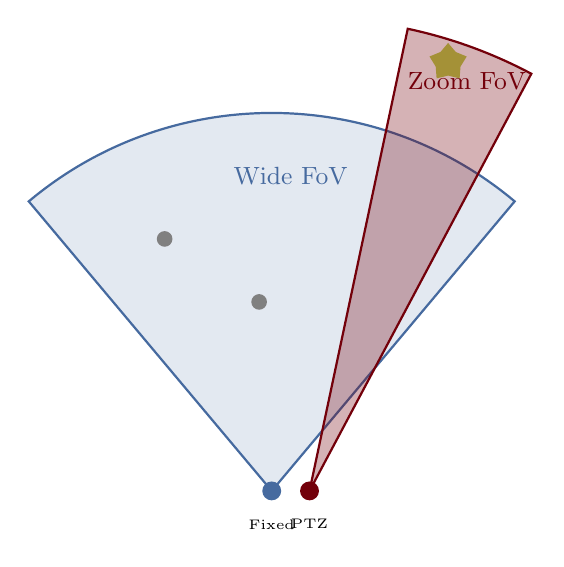
\begin{tikzpicture}[scale=0.8]
    % Cameras (simple dots, side by side)
    \fill[CBlue] (-0.3, 0) circle (0.15);
    \fill[Garnet] (0.3, 0) circle (0.15);
    \node[below, font=\tiny] at (-0.3, -0.3) {Fixed};
    \node[below, font=\tiny] at (0.3, -0.3) {PTZ};
    
    % Wide FOV (Blue) - Arc Sector
    % Center at (-0.3,0), Radius 6, Angle 50 to 130 (80 deg width)
    \draw[CBlue, thick, fill=CBlue, fill opacity=0.15] 
        (-0.3, 0) -- ++(130:6) arc (130:50:6) -- cycle;
    \node[CBlue, font=\small] at (0, 5) {Wide FoV};
    
    % Zoom FOV (Red) - Arc Sector, longer radius
    % Center at (0.3,0), Radius 7.5, Pointing at approx 70 deg
    \draw[Garnet, thick, fill=Garnet, fill opacity=0.3] 
        (0.3, 0) -- ++(78:7.5) arc (78:62:7.5) -- cycle;
    \node[Garnet, font=\small] at (2.8, 6.5) {Zoom FoV};
    
    % Target inside zoom beam
    \node[star, star points=5, fill=CGold, minimum size=0.4cm] at (2.5, 6.8) {};
    
    % Other objects in wide FOV but outside zoom
    \node[circle, fill=gray, inner sep=2pt] at (-2, 4) {};
    \node[circle, fill=gray, inner sep=2pt] at (-0.5, 3) {};
    
\end{tikzpicture}

\end{document}
